\documentclass[11pt]{article}
\usepackage[margin=1in]{geometry}
\usepackage{amsmath,amssymb,amsthm}
\usepackage{booktabs}
\usepackage{float}
\usepackage{graphicx}
\usepackage[hidelinks]{hyperref}

\newtheorem{theorem}{Theorem}
\newtheorem{proposition}{Proposition}
\newtheorem{lemma}{Lemma}
\newtheorem{corollary}{Corollary}
\theoremstyle{definition}
\newtheorem{definition}{Definition}

\newcommand{\Fp}{\mathbb{F}_p}
\newcommand{\Z}{\mathbb{Z}}
\newcommand{\Ehat}{\widehat{E}}
\newcommand{\red}{\mathrm{red}}
\newcommand{\ord}{\mathrm{ord}}
\newcommand{\Aut}{\mathrm{Aut}}
\DeclareMathOperator{\Uk}{U}

\title{\bf When a Control Does Not Control:\\
Mechanism-Derived Nulls for a False Positive\\
in $p$-adic ECDLP Cryptanalysis}

\author{W.\ T.\ Trevena\thanks{Correspondence: william.todd.trevena@gmail.com.
Code, data, and a per-phase index:
\url{https://github.com/wtrevena/ecdsa-lift} (release tag
\texttt{paper-v4}; an archival DOI will accompany the camera-ready).}}

\date{June 2026\\[2pt]
{\small Revised version (v4). Code and data:
\url{https://github.com/wtrevena/ecdsa-lift}, commit
\texttt{566a48939199cb870bc9c069696063008130dd79} (tag \texttt{paper-v4}).}}

\begin{document}
\maketitle

\begin{abstract}
Automated pipelines that fan out many structural probes against a hard
problem and surface the most anomalous are false-positive engines, in two
distinct ways: moderate separations ($\sim$$5\sigma$) are cheap under
enough multiple probing, and---more dangerously, as here---a \emph{real}
public structure tested against the \emph{wrong null} produces apparent
separations that grow without bound. This paper is a methodological case
study of one such false positive, fully dissected. In a systematic
negative exploration of $p$-adic lifting attacks on the elliptic curve
discrete logarithm problem (ECDLP), a Gowers $\Uk^2$ / Fourier analysis
of the Teichm\"uller lift error $\delta(k)$ produced a persistent
elevation, growing from $\sim$$3$ to $\approx44$ standardized units with
the curve order, that a standard value-permutation control certified as
``real, index-ordered structure.'' We show this was a \emph{control that
cannot separate the hypotheses it was meant to test}. Mechanism-derived
nulls---one per candidate explanation---localize the entire signal to a
single exact, public identity, the antisymmetry
$\delta(k)+\delta(n-k)=[n]\tau(G)$: a positive control carrying
\emph{only} that reflection reproduces the elevation and its growth, a
converse control (a genuine but non-odd section, built by kernel offsets)
collapses it at full sequence length, and a sham control (an odd kernel
offset) leaves it intact. We make the mechanism analytic: the reflection
turns each Fourier mode into an \emph{improper} complex Gaussian, and a
pseudo-variance identity classifies the $\Uk^2$ mass inflation of any
linear index constraint, with the reflection attaining the maximal factor
$3/2$ and a closed-form $\approx0.427\sqrt L$ growth law that an auditor
can apply directly. An inertness theorem---an explicit instance, in
lift-error language, of a principle of Silverman and of Gadiyar--Padma,
stated for an arbitrary abelian-group extension---explains why every such
anomaly on these curves must reduce to artifact-or-identity for
$\gcd(n,p)=1$, and the boundary is sharp: at $n=p$ the section ambiguity
is annihilated and the surviving invariant is Smart's attack. The
experiments are diagnostic, not an empirical security evaluation of
deployed curves; the reach to large-prime ECDSA-type curves is through
the theorem's generality, not through cryptographic-scale experiments.
The transferable contribution is the \emph{Mechanism-Resolved Null
Protocol}: a control is valid only against a named alternative
hypothesis, nulls must be derived from mechanisms, a positive control
must reproduce any surviving signal, a converse control should break it,
and a structural reason for inertness beats an accumulation of passed
tests.
\end{abstract}

\section{Introduction}

A recurring temptation in cryptanalysis is to lift a hard problem into a
richer setting---a $p$-adic ring, a formal group, a higher-genus
Jacobian---hoping that structure invisible over $\Fp$ becomes visible and
exploitable. For the ECDLP this hope is well mapped: Silverman's ``four
faces of lifting'' \cite{silvermanlift,silverman4faces} catalogues the
local/global $\times$ torsion/non-torsion strategies and the obstruction
each meets, and the only $p$-adic local lift that ever broke an ECDLP is
Smart's attack on anomalous curves \cite{smart,satoharaki,semaev}, where
the group order equals the characteristic.

Automating such explorations sharpens an old hazard. A pipeline that
computes many encodings of a lift invariant and reports the most unusual
will, after enough nulls, return an ``anomaly,'' and the analyst must
decide whether it is signal. We conducted a long, deliberately exhaustive
negative exploration of the canonical-lift attack surface for ordinary
curves with large prime-order subgroups---the ECDSA regime---and hit
exactly this case: a higher-order Fourier probe returned a clear
$5$--$11\sigma$ effect on the original sweep, a textbook control endorsed
it, and only a more careful experiment overturned it. The overturning, and the reason the
anomaly \emph{had} to be spurious, are the substance of this paper.

\paragraph{Contributions.}
\begin{itemize}
\item A worked, quantitative example of a \emph{control that does not
control}: a permutation test that appears to certify structure but
provably cannot separate the competing explanations
(\S\ref{sec:falsepos}).
\item \emph{Mechanism-derived controls}: enumerate the candidate
generating mechanisms and build one null per mechanism, including a
\emph{positive} control in which a synthetic model of the surviving
mechanism reproduces the statistic quantitatively, a \emph{converse}
control---a genuine section deliberately built (by kernel offsets) to
break the antisymmetry while preserving everything else, on which the
elevation collapses at full sequence length---and a \emph{sham} control
(an odd kernel offset) on which it does not (\S\ref{sec:controls}). This
localizes the anomaly (an elevation of standardized size $\sim$$3$--$14$
on the clean controlled set) to one exact public identity.
\item A closed-form account of the artifact (\S\ref{sec:controls},
Prop.~\ref{prop:pseudovar}): a pseudo-variance identity that derives the
mass-inflation factor of \emph{any} index-coupling constraint, recovering
the reflection's exact $3/2$ and the $\approx0.427\sqrt L$ growth law as
the maximal case, and predicting (via a carry model) the small residual
spectral mismatch as a falsifiable effect at $L\gtrsim 3000$.
\item An inertness theorem (\S\ref{sec:theorem}), stated for an arbitrary
abelian-group extension, explaining why such anomalies are forced: for
$\gcd(n,p)=1$ the secret-dependent part of any section lift error is
$[k]c$, governed by $k \bmod p^{e-1}$, which the public data $(E,G,Q)$
does not determine over the natural lift (and which no known efficient
algorithm computes from it---a state-of-knowledge remark, kept separate
from the theorem). We present it as the explicit instance it is of
\cite{silvermanlift,gadiyarpadma}, with proof and verification.
\item A sharp-boundary demonstration (\S\ref{sec:boundary}): the same
construction on an anomalous curve ($\gcd(n,p)=p$) recovers the secret
with $100\%$ success ($52/52$ over all nonzero residues). The theorem's
one hypothesis is exactly the line between inert and broken.
\item A scope map (\S\ref{sec:scope}): precisely which attack schema this
refutes, which it does not, and a named, checklist-form discipline---the
\emph{Mechanism-Resolved Null Protocol}---future searches should follow.
\end{itemize}

The theorem is not new mathematics; its role is to certify, after the
fact, that the methodological suspicion was structurally warranted. We
stress at the outset that the experiments are diagnostic: they expose and
explain a false positive in a lift-error statistic, they are not performed
at cryptographic sizes, and they constitute no empirical security
evaluation of any deployed ECDSA curve. The extension to ordinary
prime-order ECDSA-type curves is carried by the structural theorem, which
needs only $\gcd(n,p)=1$, not by the curve sizes tested here.

\section{Background and notation}\label{sec:background}

Let $p\ge 5$ be prime and $E/\Fp$ an elliptic curve with $\#E(\Fp)=N$.
Fix $G\in E(\Fp)$ of order $n$ with $\gcd(n,p)=1$, and $Q=kG$; the ECDLP
is to recover $k\in\Z/n\Z$ from $(E,G,Q)$. For $e\ge 1$, reduction modulo
$p$ on a fixed Weierstrass lift gives the exact sequence of abelian
groups
\begin{equation}\label{eq:ses}
0 \longrightarrow \Ehat(p\Z/p^e) \longrightarrow E(\Z/p^e)
  \xrightarrow{\ \red\ } E(\Fp) \longrightarrow 0,
\end{equation}
with kernel of reduction $\Ehat(p\Z/p^e)$ a $p$-group of order $p^{e-1}$~\cite{silvermanaec}.
The formal parameter $z=-X/Y$ identifies $\Ehat$ with $(p\Z/p^e,+_F)$
($+_F$ the formal group law), and the formal logarithm
$\log\colon\Ehat\to(p\Z/p^e,+)$ is an isomorphism with
$\log([m]u)=m\log(u)$. For $E\colon y^2=x^3+b$ the invariant differential
is $\omega=(1+3b\,z^6+\cdots)\,dz$, so
$\log(z)=z+\tfrac{3b}{7}z^7+\cdots$; for $z\in p\Z$ and $e\le 4$ the
correction vanishes ($z^7\in p^7\Z$), hence $\log(z)\equiv z\pmod{p^e}$
and kernel arithmetic is additive in $z$ at our precision.

A \emph{section} is a map $\tau\colon E(\Fp)\to E(\Z/p^e)$ with
$\red\circ\tau=\mathrm{id}$; the Teichm\"uller and Hensel lifts are
sections, generally not homomorphisms. We use the $x$-Teichm\"uller /
Hensel section throughout; it satisfies $\tau(-P)=-\tau(P)$ (the two
Hensel roots in $y$ are negatives), a property we invoke once below. The
\emph{lift error} (a $1$-cochain valued in $\Ehat$ by \eqref{eq:ses}) is
\begin{equation}
\delta_\tau(k)\ :=\ [k]\,\tau(G)\ -\ \tau(kG)\ \in\ \Ehat(p\Z/p^e).
\end{equation}
We write $\delta(k)$ for the Teichm\"uller case and
$z(\delta(k))\in p\Z/p^e$ for its formal parameter; for an integer
$z\in\Z/p^e$, $\mathrm{digit}_j(z)$ is the coefficient of $p^j$ in the
base-$p$ expansion (digit $0$ is the units place, identically $0$ here
since $z\in p\Z$).

\begin{table}[h]
\centering\small
\begin{tabular}{ll}
\toprule
Symbol & Meaning\\
\midrule
$\delta_\tau(k)=[k]\tau(G)-\tau(kG)$ & lift error of section $\tau$ (in $\Ehat$); $\delta$ = Teichm\"uller case\\
$z(\delta(k))\in p\Z/p^e$ & formal parameter $-X/Y$ of $\delta(k)$; additive on $\Ehat$ at $e\le4$\\
$\mathrm{digit}_j(z)$ & coefficient of $p^j$ in the base-$p$ expansion of $z$\\
$f_j(k)=e^{2\pi i\,\mathrm{digit}_j(z(\delta(k)))/p}$ & phase encoding of digit $j$, $k=1,\dots,n-1$\\
$\|f\|_{\Uk^2}^4=\sum_\xi|\hat f(\xi)|^4$ & $\Uk^2$ \emph{mass} (mean $2/L$, SD $\Theta(L^{-3/2})$ under i.i.d.)\\
$\|f\|_{\Uk^2}=(\text{mass})^{1/4}$ & $\Uk^2$ \emph{norm} (SD $\Theta(L^{-3/4})$ under i.i.d.)\\
$C_n=z([n]\tau(G))$ & antisymmetry constant of \eqref{eq:antisym}; public\\
\bottomrule
\end{tabular}
\caption{Notation. The mass/norm distinction matters for standardized
effect sizes (Prop.~\ref{prop:scaling}).}
\label{tab:notation}
\end{table}

\paragraph{Prior art.} That a $p$-adic lift transports the ECDLP without
weakening it, that the canonical (Teichm\"uller) lift carries no
information, and that ``solving the DLP is equivalent to constructing a
non-canonical lift'' are due to Silverman \cite{silvermanlift,
silverman4faces} for elliptic curves and to Gadiyar--Maini--Padma and
Gadiyar--Padma \cite{gadiyarpadma} for $\Fp^\times$. Smart, Satoh--Araki
and Semaev \cite{smart,satoharaki,semaev} give the anomalous attack; the
canonical lift is Lubin--Serre--Tate \cite{lst}, its computational
instance Satoh's point counting \cite{satohcount}. Yasuda \cite{yasuda}
studies the ECDLP transported to the $p$-adic field and to formal groups,
where the formal logarithm makes the kernel DLP easy yet an $\Fp$
instance gains nothing---consistent with, and adjacent to, the inertness
mechanism here. Our theorem repackages these in the lift-error language.
On the methodology side, the principles we import are textbook in spirit:
permutation tests are valid only under exchangeability with respect to
the null being tested \cite{good}, negative and positive controls
diagnose miscalibrated nulls \cite{lipsitch}, and unacknowledged analytic
flexibility manufactures separations
\cite{gelmanloken,simonsohn,steegen}; randomness-test batteries in
cryptography have their own calibration pitfalls \cite{nistsp}. The
contribution is not these principles but their disciplined import into an
automated cryptanalytic workflow, with the failure dissected to the
constant.

\section{The exploration, in brief}\label{sec:exploration}

The full study ran forty-seven numbered phases against the canonical-lift /
formal-group attack surface for $j=0$ (CM by $\Z[\omega]$) and generic
ordinary curves; Appendix~\ref{app:phases} indexes them. Probes included
pseudorandomness of $\delta$ (DFT flatness, maximal Berlekamp--Massey
complexity, uniform $p$-adic valuation, no polynomial/Mahler/%
multiplicative fit); a homomorphic section from $H^2$ vanishing (which
exists but, being a homomorphism, annihilates the attack); an explicit
Serre--Tate canonical lift validated by $\delta_{\mathrm{can}}\equiv 0$;
HNP/lattice (LLL, BKZ) attacks on the cocycle; MOV embedding degree;
ordinary/supersingular bridges; genus-$2$ Jacobian covers; Weil pairings;
Iwasawa $\mu$; and a Frobenius/unit-root analysis. Every one was inert.
Two exact relations survived, both \emph{public} (computable from the
curve alone) and both giving no advantage: an automorphism-equivariance
of the leading $\delta$-digit, and the antisymmetry
\begin{equation}\label{eq:antisym}
\delta(k)+\delta(n-k)=[n]\,\tau(G),
\end{equation}
which holds for any section with $\tau(-P)=-\tau(P)$ (so that
$\tau(kG)+\tau(-kG)=O$), and which we confirmed holds \emph{exactly} in
the $z$-coordinate---e.g.\ for $p=97$ ($n=79$; a curve distinct from the
$p=67$, $n=79$ entry of Table~\ref{tab:p43}),
$z(\delta(k))+z(\delta(n-k))$ takes a single value across all $39$
reflection pairs $(k,n-k)$. We emphasize that \eqref{eq:antisym} encodes
nothing beyond the familiar negation symmetry $Q\leftrightarrow-Q$ (i.e.\
$k\leftrightarrow n-k$): it halves the search space, as every implementor
already knows, and confers no further advantage.

\section{A false positive: the Gowers anomaly}\label{sec:falsepos}

Encode digit $j$ of the lift error as a phase,
$f_j(k)=\exp\!\big(2\pi i\,\mathrm{digit}_j(z(\delta(k)))/p\big)$ for
$k=1,\dots,n-1$, and measure the Gowers $\Uk^2$ norm~\cite{taovu} against an
$S^1$-uniform random baseline (definitions and counts in
\S\ref{sec:stats}). Across many primes the $\Uk^2$ norm was elevated
$5$--$11\sigma$ on the original exploratory sweep (Phase 37, a mixed bag
of curves later found to include supersingular and anomalous cases); on
the clean controlled set of \S\ref{sec:controls} the elevation is
$\sim$$3$--$14\sigma$ ($z(\text{real vs rand})$ ranges $3.3$ to $13.6$).
$\Uk^3$ and higher sat at baseline. The leading Fourier
coefficient decayed as $|\hat f(\alpha)|\sim C n^{-\beta}$ with
$\beta<1/2$, on CM, $j{=}1728$, and non-CM curves alike. An internal
report concluded this was a genuine, previously unnoticed degree-$1$
structural property of the Teichm\"uller cocycle ``not explained by any
universal identity.''

The evidence offered was a permutation control: randomly permuting the
\emph{values} of $f_j$ destroyed the elevation, read as proof that the
structure lived in the index ordering, hence was ``real.'' This inference
is invalid, and seeing why is the point of the paper.

\section{Mechanism-derived controls}\label{sec:controls}

\paragraph{The principle.} A control is a null model, and a null tests
exactly one alternative: the one under which the statistic is recomputed.
The value-permutation control recomputes $\Uk^2$ under ``the multiset of
digit values, in random order,'' so it separates ``structure in the value
distribution'' from ``structure in the ordering''---and nothing else. But
at least three mechanisms predict ordered structure here, and the
permutation kills all three at once, so it cannot attribute the signal to
any one:
\begin{enumerate}
\item[(H1)] \emph{Prefix-sum artifact.} $\delta(k)=-\sum_{i<k}c(iG,G)$ is
a running sum; summation is a low-pass filter
($\hat s(\xi)=\hat d(\xi)/(1-e^{2\pi i\xi/n})$, a $1/\xi$ pole at
$\xi=0$), so \emph{any} increments with this multiset, once summed, carry
elevated low-frequency $\Uk^2$.
\item[(H2)] \emph{Antisymmetry shadow.} The exact reflection
\eqref{eq:antisym} couples Fourier mode $\alpha$ with $-\alpha$, a rigid
constraint that elevates $\Uk^2$.
\item[(H3)] \emph{Genuine new structure}, the claimed explanation.
\end{enumerate}
We build one null per mechanism, each derived from how that mechanism
generates ordering. All numbers below are on the clean ordinary set of
Table~\ref{tab:p43} (Phase 43), under the pre-registered protocol of
\S\ref{sec:stats}.

\paragraph{H1 (increment shuffle).} $s(k)=z(\delta(k))$ is the exact
cumulative sum of its first differences $d(k)=s(k+1)-s(k)$. Shuffle $d$,
re-sum in the new order, recompute $\Uk^2$; the increment multiset is
identical, only the order changes. The shuffled-increment prefix sums sit
\emph{at} the random baseline ($z(\text{incShuf vs rand})\in[-0.3,+0.5]$
on every curve), while the true ordering sits $+3.5$ to $+12.5$ above
them, growing with $n$ (Table~\ref{tab:p43}, cols.\ 4--5). H1 is refuted:
the digit nonlinearity destroys the walk's low-frequency mass, so the
signal is in the \emph{specific} order, not in summation.

\paragraph{H2 (half-sequence).} The reflection \eqref{eq:antisym} relates
each $k$ to $n-k$. On the first half $k=1,\dots,\lfloor(n-1)/2\rfloor$
every reflection partner lies outside the window, so H2 predicts no
internal constraint there while H3 predicts the signal persists.
Re-running the increment-shuffle control on the half collapses the
elevation to noise ($z(\text{half vs incShuf})\in[-1.3,+1.5]$, no growth
in $n$; Table~\ref{tab:p43}, col.\ 6).

\paragraph{H2, positive control (the decisive test).} Absence of signal
on the half is necessary but not sufficient. We therefore test H2
\emph{constructively}: generate synthetic sequences that impose
\emph{only} the reflection, $s(k)$ i.i.d.\ uniform on the first half and
$s(n-k)=C-s(k)$ with $C=z([n]\tau(G))$, carrying no other structure, and
measure their $\Uk^2$. If reflection alone is the mechanism, these must
reproduce the real statistic. They do, quantitatively: the synthetic
$\Uk^2$ is elevated $+3.8$ to $+12.5$ over the random baseline---tracking
the real elevation across the whole range of $n$---and the real sequences
are statistically indistinguishable from them
($z(\text{real vs syn})\in[-1.4,+1.5]$; Table~\ref{tab:p43}, cols.\
7--8). The match on the $\Uk^2$ elevation and its growth with $n$ is the
substance of the positive control, and it is exact (cols.\ 7--8). The
finer digit-dependent Fourier decay is only \emph{partially} reproduced:
fitting $|\hat f|\sim C n^{-\beta}$ across the seven curves, the real
sequences give $\beta_{\mathrm{real}}\approx\{0.34,0.45,0.36\}$ for
digits $1,2,3$, whereas the reflection-only synthetic draws give a nearly
flat $\beta_{\mathrm{syn}}\approx\{0.41,0.41,0.40\}$. Reflection alone
thus reproduces the overall power-law decay ($\beta\approx0.4$, the same
order as the real exponents) but not its digit-to-digit variation; we do
\emph{not} claim the spectra match in detail. The residual
digit-to-digit variation is, however, consistent with finite-size fit
scatter rather than secondary structure: resampling the seven-curve fit
on reflection-only sequences gives $\beta_{\mathrm{syn}}$ with mean
$\approx0.40$ and standard deviation $\approx0.06$ \emph{with no digit
dependence built in}, and each real exponent $\{0.34,0.45,0.36\}$ lies
within $\approx1$ standard deviation of that mean. The mild downward
spread of the interior-digit exponents is moreover the \emph{sign}
predicted by the carry model of \S\ref{sec:controls}
(Prop.~\ref{prop:scaling}): digit~$1$ reflects exactly while digits $2,3$
carry a small borrow-induced deficit. Under the standard assumption that
the ECDLP is hard on these curves, the residual cannot be cryptanalytic in
any case---it is a deterministic post-processing of the public digit map
of a public object (Theorem~\ref{thm:main}, Corollary~\ref{cor:main} and
the Consequence following it)---so
we do not pursue it further; the decisive evidence that H2 is the
mechanism is the $\Uk^2$ match, which is genuine. A post-hoc confirmatory
run on a large-prime-order curve ($p=10477$, $n=10639$ prime; Phase 47,
last row of Table~\ref{tab:p43}) extends the pattern by more than an order
of magnitude in $n$: the real elevation reaches $+43$--$44$, the
reflection-only synthetics track it at $+44.5$--$44.8$, and real vs.\
synthetic stays within $\pm2.1$.

\paragraph{The converse control (breaking the reflection).} A positive
control can be accused of circularity---a synthetic sequence built with
the reflection will of course exhibit the reflection statistic. The
decisive converse is to remove the reflection from the \emph{real}
construction and check that the elevation disappears. The antisymmetry
\eqref{eq:antisym} holds only because the section is odd,
$\tau(-P)=-\tau(P)$; the converse must therefore break oddness
\emph{while remaining a genuine section}, so that nothing else changes.
(A first attempt, Phase~49, chose the Hensel $y$-root by a
negation-insensitive ``smaller integer representative'' rule; that rule
is \emph{not} a section---it lifts $-P$ rather than $P$ on roughly half
the points, so half the lift errors leave the kernel of reduction and the
degeneracy filter halves the usable length. The collapse it showed was
therefore confounded, as Phase~49b documented; we retain it only as a
cautionary record.) The clean construction perturbs the odd section by a
\emph{kernel offset}:
\[
\tau'(P)\ :=\ \tau(P)\ +\ [h(P)]\,K_1,\qquad
K_1:=[n]\tau(G)\in\Ehat,\quad h\colon E(\Fp)\to\Z/p^{e-1},
\]
where $h$ is a deterministic function of the point. Because the offset
lies in the kernel, $\red\circ\tau'=\mathrm{id}$ for \emph{every} $P$:
$\tau'$ is a genuine section, $\delta_{\tau'}(k)$ stays in the kernel for
all $k$, and the usable length is the full $n-1$ with zero drops. Oddness
fails exactly when $h$ is not odd, and in $z$-coordinates the new lift
error is computable in closed form,
$z(\delta'(k))=z(\delta(k))+(k\,h(G)-h(kG))\,C_n \bmod p^e$. The result
(Phase~60, same curves, same secrets, same encoding) is a double
dissociation. With non-odd offsets ($h(P)=x(P)$ or $h(P)=x(P)+7y(P)$
mod $p^{e-1}$): the antisymmetry sum $z(\delta'(k))+z(\delta'(n-k))$
ceases to be single-valued ($\lfloor(n-1)/2\rfloor$ distinct values, one
per pair), and the $\Uk^2$ elevation collapses from $z(\text{real vs
rand})$ of $+3.6,+6.6,+11.8,+45.9$ (digit-$1$ values across
$p=67,211,823,10477$) to baseline ($z\in[-1.6,+1.9]$ across all curves
and digits). With an \emph{odd} offset ($h(P)=y(P)$, a sham control for
which $\tau'$ remains odd): the identity remains single-valued and the
elevation remains ($+3.4,+4.7,+9.5,+47.8$ at digit~$1$). Breaking oddness
destroys identity and elevation together; preserving oddness under an
equally disruptive kernel perturbation preserves both. The mechanism is
the reflection---and nothing else about $\delta$.

\paragraph{The growth law is itself an artifact signature.} The elevation
does not merely persist with $n$; it \emph{grows}, from $\sim3$ at $n=79$
to $\sim44$ at $n=10639$. It is tempting to read growth-with-$n$ as
accumulating signal---this is precisely what the internal Phase-37 report
did. The opposite is true: the growth is forced by the reflection alone
and carries no curve information, as the following closed form shows.

We treat the general mechanism first and read off the reflection as the
extremal case. Write the $\Uk^2$ mass as
$\|f\|_{\Uk^2}^4=\sum_\xi|\hat f(\xi)|^4$ with
$\hat f(\xi)=\tfrac1L\sum_k f(k)e^{-2\pi ik\xi/L}$. In the large-$L$ limit
each nonzero mode $Z_\xi:=\hat f(\xi)$ is a mean-zero complex Gaussian
characterized by two second moments: the \emph{variance}
$\sigma^2=\mathbb E|Z_\xi|^2=1/L$ and the \emph{pseudo-variance}
$\rho(\xi)=\mathbb E[Z_\xi^2]$, the latter zero for a proper
(circularly symmetric) mode and nonzero exactly when a constraint couples
$\xi$ to $-\xi$.

\begin{proposition}[Pseudo-variance classification of $\Uk^2$
inflation]\label{prop:pseudovar}
For a complex Gaussian $Z$ with variance $\sigma^2$ and pseudo-variance
$\rho$,
\begin{equation}\label{eq:fourth}
\mathbb E|Z|^4=2\sigma^4+|\rho|^2 .
\end{equation}
Hence for $f\colon\Z/L\to S^1$ whose modes have per-mode pseudo-variance
$\rho(\xi)$,
$\mathbb E\big[\|f\|_{\Uk^2}^4\big]
=\big(2+\langle|\rho|^2\rangle/\sigma^4\big)/L+o(1/L)$, where
$\langle\cdot\rangle$ averages over the $L-1$ nonzero modes, and the
mass-inflation factor relative to the i.i.d.\ baseline is
\begin{equation}\label{eq:infl}
\text{INFLATION}\;=\;1+\frac{\langle|\rho(\xi)|^2\rangle}{2\sigma^4}\;\in\;[1,\tfrac32].
\end{equation}
The upper bound $|\rho|\le\sigma^2$ (Cauchy--Schwarz) is attained, giving
the maximal $3/2$, \emph{iff} $|\rho(\xi)|=\sigma^2$ a.e.---the case of an
index-reversing constraint $\hat f(-\xi)=\beta\,\overline{\hat f(\xi)}$;
a constraint that fixes each mode (e.g.\ a translation $k\mapsto k+s$)
gives $\rho\equiv0$ and no inflation.
\end{proposition}

\begin{proof}
Write $Z=X+iY$ with real covariance $\big(\begin{smallmatrix}a&c\\
c&b\end{smallmatrix}\big)$, so $\sigma^2=a+b$ and $\rho=(a-b)+2ic$,
$|\rho|^2=(a-b)^2+4c^2$. Isserlis' theorem gives $\mathbb E[X^4]=3a^2$,
$\mathbb E[Y^4]=3b^2$, $\mathbb E[X^2Y^2]=ab+2c^2$, whence
$\mathbb E|Z|^4=\mathbb E[(X^2+Y^2)^2]=3a^2+3b^2+2ab+4c^2
=2(a+b)^2+(a-b)^2+4c^2=2\sigma^4+|\rho|^2$, proving \eqref{eq:fourth}.
Summing over modes and using $\sigma^2=1/L$ gives the mass and
\eqref{eq:infl}; the bound $|\rho|\le\sigma^2$ is Cauchy--Schwarz on
$\mathbb E[Z^2]$ versus $\mathbb E|Z|^2$. The index-reversing constraint
forces $Z_{-\xi}=\beta\,\overline{Z_\xi}$, hence
$\mathbb E[Z_\xi^2]$ has modulus $\mathbb E|Z_\xi|^2=\sigma^2$; a constraint
fixing each mode leaves $\mathbb E[Z_\xi^2]=0$.
\end{proof}

\begin{proposition}[The reflection inflates the $\Uk^2$ mass by a
limiting factor of exactly $3/2$]\label{prop:scaling}
Let $f\colon\Z/L\to S^1$ be subject to \emph{only} the antisymmetry
constraint $f(L{+}1{-}k)=\beta\,\overline{f(k)}$ ($\beta\in S^1$ fixed, the
free half i.i.d.\ $S^1$-uniform)---the reflection-only synthetic of the
positive control. Then $\mathbb E\big[\|f\|_{\Uk^2}^4\big]=3/L+o(1/L)$,
versus $2/L+o(1/L)$ for i.i.d.\ $S^1$-uniform entries; the limiting mass
ratio is exactly $3/2$, independent of the value alphabet. The
standardized synthetic-vs-random gap, measured on the $\Uk^2$
\emph{norm} against the i.i.d.\ null, is
$z(\mathrm{syn/rand})=2^{7/4}\big(3^{1/4}-2^{1/4}\big)\sqrt L+o(\sqrt L)
\approx0.427\sqrt L$.
\end{proposition}

\begin{proof}
\emph{Mean.} The constraint is index-reversing, so by
Prop.~\ref{prop:pseudovar} the inflation factor is $3/2$, i.e.\
$\mathbb E[\|f\|_{\Uk^2}^4]=3/L+o(1/L)$. The finitely many exceptional
modes (the zero mode, whose magnitude is $O_P(L^{-1})$ in mass either
way; the self-paired mode $\xi=L/2$ for even $L$; the fixed physical
midpoint for odd $L$) each contribute $O(1/L^2)$ to the mass and are
absorbed in the $o(1/L)$.

\emph{Variance of the i.i.d.\ mass---the step that fixes the constant.}
Write $M=\sum_\xi p_\xi^2$ with $p_\xi=|\hat f(\xi)|^2$. Parseval forces
$\sum_\xi p_\xi=\tfrac1L\sum_k|f(k)|^2=1$ \emph{exactly}, so the
periodogram is a random point on the simplex; for random phases it is
asymptotically a uniform $\mathrm{Dirichlet}(1,\dots,1)$ vector on $L$
parts, \emph{not} a vector of independent exponentials. The Dirichlet
moment formula
$\mathbb E[\prod_i p_i^{a_i}]=\prod_i a_i!\cdot\Gamma(L)/\Gamma(L+\sum
a_i)$ gives
\[
\mathbb E[M]=\frac{2}{L+1},\qquad
\mathbb E[M^2]=\frac{4(L+5)}{(L+1)(L+2)(L+3)},\qquad
\operatorname{Var}(M)=\frac{4}{L^3}+O(L^{-4}).
\]
Ignoring the Parseval constraint would give
$\operatorname{Var}(M)=L\cdot\operatorname{Var}(|Z|^4)=20/L^3$ (since
$\operatorname{Var}(|Z|^4)=20\sigma^8$ for a proper complex Gaussian)
and hence a growth constant $\approx0.19$, contradicting experiment; the
constraint reduces the variance by exactly the factor $5$. So
$\mathrm{SD}(M)=2L^{-3/2}+O(L^{-2})$, and by the delta method on the
\emph{norm} $M^{1/4}$ (mean $(2/L)^{1/4}$),
$\mathrm{SD}(\text{norm})=\tfrac14(2/L)^{-3/4}\cdot 2L^{-3/2}
=2^{-7/4}L^{-3/4}$.

\emph{Standardized gap.} The mean gap in the norm is
$(3/L)^{1/4}-(2/L)^{1/4}=(3^{1/4}-2^{1/4})L^{-1/4}$; dividing by
$2^{-7/4}L^{-3/4}$ gives $2^{7/4}(3^{1/4}-2^{1/4})\sqrt L$.
\end{proof}

The exact Dirichlet computation and a Monte Carlo confirmation that
$\operatorname{Var}(M)$ tracks $4/L^3$ (and not $20/L^3$) across
$L\in[78,3000]$, together with the delta-method check
$\mathrm{SD}(\text{norm})/2^{-7/4}L^{-3/4}\in[0.96,1.01]$, are Phase~61.

The coefficient $2^{7/4}(3^{1/4}-2^{1/4})=0.4267\ldots$ is fully analytic;
it is the closed form of the constant the original sweep had only
measured. Standardizing the $\Uk^2$ \emph{norm} against the
empirical-null standard deviation, we confirmed it $p$- and
$L$-independent across $L\in[78,10^6]$ (Phases~48, 56): the mass ratio
holds to $1.500$ at $L=10^6$, and $0.427\sqrt n$ reproduces the syn/rand
column of Table~\ref{tab:p43} and the Phase-47 value (predicted $44.8$
vs.\ observed $44.6$ at $n=10639$) within finite-size noise. So $\sqrt n$
growth is the \emph{signature of the antisymmetry artifact}, not of an
accumulating signal---the exact inference the original report inverted.
Equation~\eqref{eq:infl} also makes the discriminator quantitative: a
constraint sending mode $\xi$ to its reversal $-\xi$ inflates the mass to
$3/L$, whereas one sending it elsewhere (e.g.\ the fixed-shift involution
$k\mapsto k+L/2$) leaves it at $2/L$; we verified both numerically (ratios
$1.499$ vs.\ $1.001$; Phase~55), so an auditor reads the mechanism off the
constraint's action on Fourier indices. Figure~\ref{fig:artifact}
summarizes the evidence: the separated null distributions, the
$0.427\sqrt L$ law against the data, and the hypothesis-by-control matrix
whose first row is the permutation control's failure.

\begin{figure}[t]
\centering
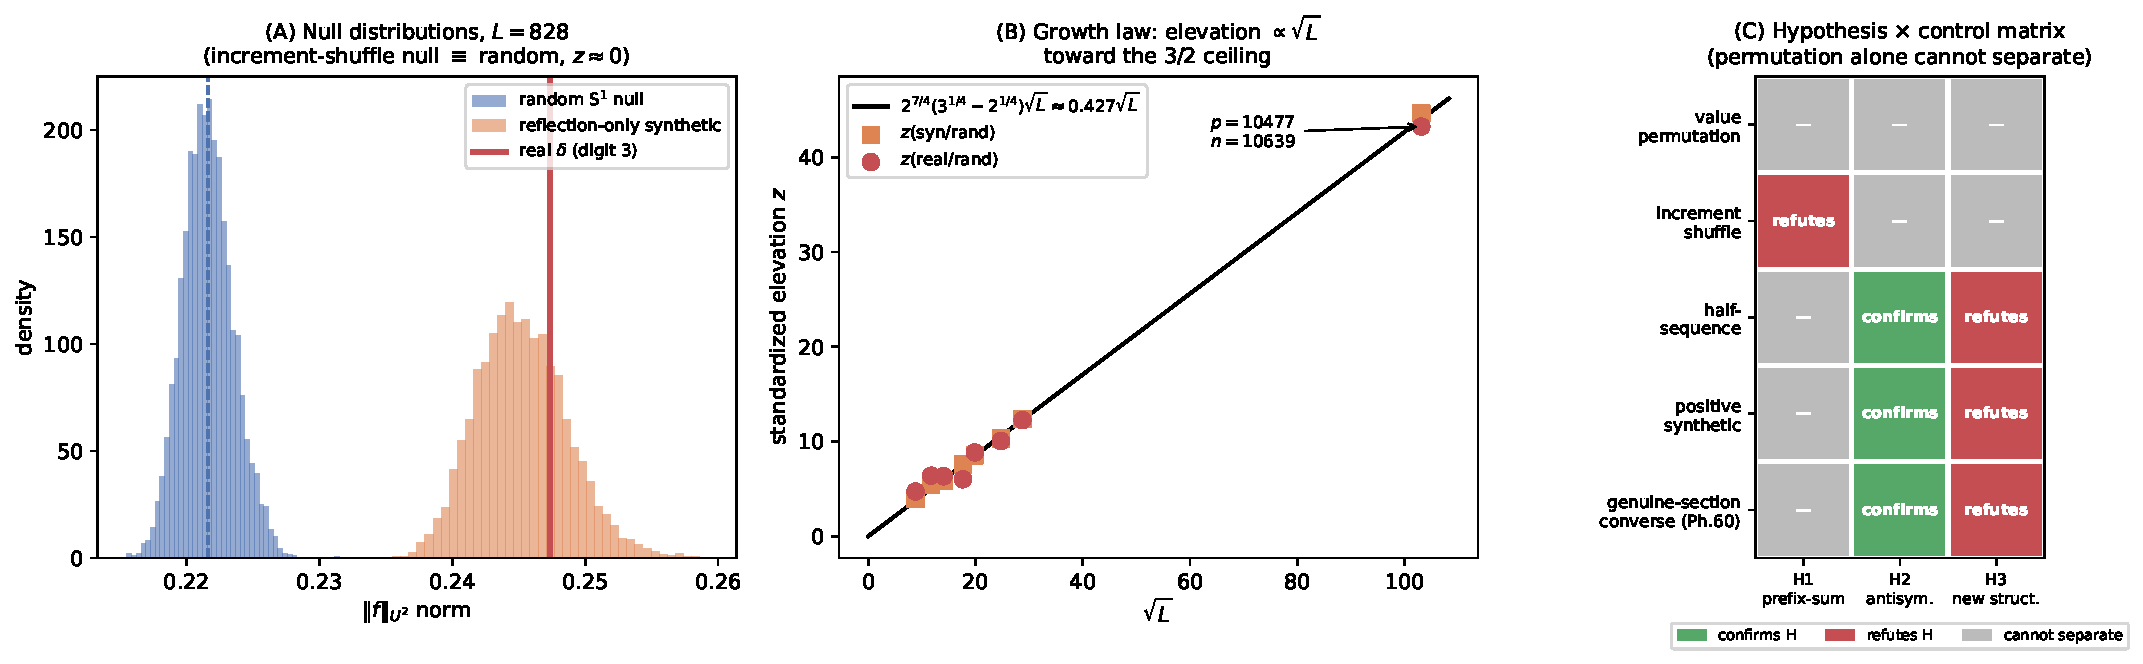
\includegraphics[width=\linewidth]{fig_artifact.pdf}
\caption{(A)~Null distributions of the $\Uk^2$ norm at $L=828$: the
$S^1$-random baseline, the reflection-only synthetic, and the measured
real value (digit~$3$); the increment-shuffle null coincides with the
random null ($z\approx0$ on every curve). (B)~Standardized elevation
versus $\sqrt L$ for the seven clean curves and the confirmatory
$p=10477$: both $z(\text{syn/rand})$ and $z(\text{real/rand})$ follow the
closed-form $2^{7/4}(3^{1/4}-2^{1/4})\sqrt L$ line of
Prop.~\ref{prop:scaling}. (C)~Hypothesis~$\times$~control matrix: the
value-permutation control kills all three mechanisms at once and so
separates none; each mechanism-derived control implicates or refutes a
named hypothesis, and the genuine-section converse (Phase~60) completes
the attribution. Generated by Phase~62 from committed results.}
\label{fig:artifact}
\end{figure}

\paragraph{Higher norms, and a carry prediction.} Two consequences of the
same analysis sharpen the picture. First, the inflation is a purely
second-order (quadratic-mass) phenomenon: heuristically, the extra
difference operator defining $\Uk^3$ couples reflection partners only on
an $O(1/L)$ fraction of shift--position pairs, so
$\mathbb E\|f\|_{\Uk^3}^8$ should sit at the unconstrained baseline up to
$O(1/L)$. We state this as a counting heuristic rather than a proof, and
confirm it numerically: the $\Uk^3$ excess decays as $1/L$ while the
$\Uk^2$ ratio holds at $3/2$ (Phase~59). This accounts for the otherwise
unexplained observation that $\Uk^3$ and higher sat at baseline. Second,
the real digit sequence reflects only approximately: base-$p$ borrows
mean the phase-level reflection
$\mathrm{digit}_j(C-s)\leftrightarrow\mathrm{digit}_j(s)$ holds for a
fraction $1-q_j$ of pairs. A simple independence model for the borrow
failures---a modelling assumption, not a derived fact---predicts per-mode
$|\rho|=(1-q_j)\sigma^2$, hence by \eqref{eq:infl} a mass
$\big(2+(1-q_j)^2\big)/L$. Digit $1$ reflects \emph{exactly} ($q_1=0$,
since $z(\delta)\in p\Z$ forces digit $0$ to vanish on both sides, so no
borrow reaches position $1$); interior digits have $q_2,q_3\approx0.2$
measured on the clean set---a value that depends on the constant $C$, the
digit distribution, $p$, and the sample, and is not claimed to be
universal---predicting a mild mass deficit there. At the
clean-set sizes this deficit ($\sim0.3$ in $L\cdot$mass) sits at the
$\lesssim2\sigma$ resolution limit and is \emph{not} yet distinguishable
from finite-size scatter---consistent with the small
$\beta_{\mathrm{real}}$ spread we report below---so we state it as a
falsifiable prediction: a confirmatory run at $L\gtrsim3000$ should resolve
$\Uk^2$ masses of $\approx3.0$ at digit $1$ and $\approx2.7$ at digits
$2,3$ (Phase~58).

\paragraph{Verdict.} The anomaly is the Fourier-domain shadow of the
exact, public identity \eqref{eq:antisym}: H2, not H1 or H3. It is real
but not new, and---being a public consequence of the curve's geometry
that yields only a $2$-to-$1$ search reduction---carries no cryptanalytic
advantage. The varying ``decay exponent'' and its apparent curve-family
dependence in the internal report are finite-size scatter around a single
reflection-induced spectrum; nothing family-specific survives. To rule out
a complex-multiplication artifact---the clean set is $j{=}0$, which carries
extra automorphisms---we re-ran the full protocol on $j{=}1728$ and on
generic non-CM curves ($j\in\{6,316,446\}$, prime order, $\gcd(n,p)=1$):
the $3/2$ inflation, the syn/rand tracking, and the real-vs-syn
equivalence reproduce identically, confirming the mechanism is the
antisymmetry and not the CM structure (Phase~50).

\begin{table}[t]
\centering
\small
\begin{tabular}{rrrrrrrr}
\toprule
& & & \multicolumn{3}{c}{negative controls ($z$)} & \multicolumn{2}{c}{positive ($z$)}\\
\cmidrule(lr){4-6}\cmidrule(lr){7-8}
$p$ & $n$ & $L$ & real/inc & inc/rand & half/inc & syn/rand & real/syn\\
\midrule
 67 &  79 &  78 & $+3.5..6.7$  & $-0.3..0.2$ & $-0.6..1.5$ & $+3.8..4.1$  & $-0.4..1.2$\\
163 & 139 & 138 & $+3.7..7.4$  & $+0.0..0.5$ & $-0.4..1.0$ & $+5.4..5.4$  & $-0.9..1.5$\\
211 & 199 & 198 & $+5.1..7.8$  & $+0.1..0.3$ & $-0.8..0.5$ & $+5.8..5.9$  & $-0.3..0.8$\\
349 & 313 & 312 & $+5.4..7.1$  & $-0.0..0.1$ & $-1.3..0.2$ & $+7.5..7.6$  & $-1.4..-0.4$\\
433 & 397 & 396 & $+8.2..9.6$  & $-0.1..0.2$ & $-0.4..0.6$ & $+8.4..8.6$  & $-0.1..0.7$\\
577 & 613 & 612 & $+7.8..11.5$ & $+0.1..0.2$ & $-0.5..1.1$ & $+10.2..10.4$& $-1.2..0.8$\\
823 & 829 & 828 & $+10.5..12.5$& $+0.1..0.2$ & $-0.9..0.0$ & $+12.2..12.5$& $-0.9..0.7$\\
\midrule
10477$^\dagger$ & 10639 & 10638 & $+42.7..44.1$ & $-0.0..0.0$ & $-1.1..1.8$ & $+44.5..44.8$ & $-2.0..0.7$\\
\bottomrule
\end{tabular}
\caption{Phase 43, clean ordinary $j{=}0$ curves $y^2=x^3+7$
($p\equiv 1\bmod 3$, $n=\#E(\Fp)$ prime, so $\gcd(n,p)=1$ and the curve
is neither supersingular nor anomalous); $L$ is the number of usable
$k\in[1,n-1]$ after the pre-registered degeneracy filter
(\S\ref{sec:stats}); here $L=n-1$ (no drops). Ranges are over digits
$j=1,2,3$. Negative controls: shuffling increments leaves $\Uk^2$ at the
random baseline (inc/rand) and the true ordering far above it (real/inc),
which vanishes on the half (half/inc). Positive control: synthetic
reflection-only sequences reproduce the elevation (syn/rand) and the real
sequences match them (real/syn). The entire effect is the antisymmetry
\eqref{eq:antisym}. The last row ($\dagger$, Phase 47, $p=10477$) is a
post-hoc confirmatory run under the identical protocol, reported
separately from the pre-registered seven-curve set.}
\label{tab:p43}
\end{table}

\section{Statistical protocol}\label{sec:stats}

All quantities in \S\ref{sec:controls} follow one pre-registered protocol
(fixed before the clean re-run; seed $20260609$). Precision $e=4$; digits
$j\in\{1,2,3\}$. The $S^1$-random baseline draws $300$ sequences
$g(k)=e^{i\theta_k}$, $\theta_k$ uniform on $[0,2\pi)$, of the same length
$L$; ``$\sigma$'' and ``$z$'' are the standard deviation and standardized
deviation \emph{of the relevant null}: incShuf uses $300$ increment
shuffles, syn uses $300$ synthetic draws, rand uses the $300$ baselines.
The Gowers $\Uk^2$ is computed exactly by its FFT formula. \emph{Exclusion
rule (pre-specified):} a value $z(\delta(k))$ is dropped iff its
projective lift is degenerate---$Y$ a non-unit, or $z\not\equiv 0\bmod p$
(a kernel element must have $z\equiv 0$); these are arithmetic failures of
the pure-Python lift, flagged automatically, and on the clean ordinary set
none occurred ($L=n-1$ throughout). The clean set is the seven ordinary
$j{=}0$ curves $y^2=x^3+7$ with $p\equiv 1\bmod 3$ and $n=\#E(\Fp)$ prime
(hence $\gcd(n,p)=1$, neither supersingular nor anomalous); the smallest
has $n=79$, so $L\ge 78$ throughout. No further size-based filter is
applied---every such curve in the run is reported.
We make no multiplicity correction and therefore do \emph{not} claim
discovery from any single elevated $\Uk^2$; the paper's logic is the
opposite---every elevation is traced to a named mechanism and shown to be
identity-or-artifact, and the controls are designed to \emph{remove}
signal, not to find it. Phase 47 repeats this protocol verbatim on one
large-prime-order curve ($p=10477$, $n=\#E(\Fp)=10639$ prime); being
post-hoc, it is reported separately (marked $\dagger$ in
Table~\ref{tab:p43}). Throughout, $z$-values are standardized effect
sizes against $300$-draw empirical nulls, not calibrated Gaussian tail
probabilities; we use them only comparatively, never as discovery
statistics.

\paragraph{Calibration.} Three checks make the evidential language
precise. (i) \emph{Look-elsewhere.} The exploration spans $\sim$$47$
phases $\times$ $3$ digits $\times$ $8$ curves $\times$ several encodings;
the expected maximum $|z|$ of a generic random baseline over a battery of
this size is $\approx3.2$--$3.6$ by extreme-value theory, and an empirical
$10$-statistic battery on i.i.d.\ surrogates reached $|z|=5.0$ (Phase~54).
A ``$5\sigma$'' separation from a generic baseline is therefore
\emph{expected} under this much exploration. But look-elsewhere
arithmetic explains only the moderate outliers; it cannot manufacture the
$11$--$44$ range. Those are \emph{wrong-null} false positives: a real,
public algebraic identity tested against a generic random baseline
produces a separation that grows without bound ($\propto\sqrt L$,
Prop.~\ref{prop:scaling}) while carrying no secret information. The two
mechanisms require different defenses---multiplicity control for the
first, mechanism-derived nulls for the second---and conflating them is
itself a failure mode. (ii)
\emph{Equivalence, not absence of significance.} For the real-vs-synthetic
comparison we report a two-one-sided-test bound, specified as follows:
the statistic is the $\Uk^2$ \emph{norm}; the null is the $300$-draw
reflection-synthetic distribution (mean $\mu_{\mathrm{syn}}$, SD
$s_{\mathrm{syn}}$); each digit is tested separately; and the excluded
residual is the $95\%$ one-sided upper confidence limit
$\Delta_{\mathrm{excl}}=(\max(0,z_{\mathrm{obs}})+1.645)\,s_{\mathrm{syn}}$
on any non-reflection (``H3'') component beyond the synthetic baseline,
reported as a fraction of the elevation
$E=\Uk^2_{\mathrm{real}}-\mu_{\mathrm{rand}}$. This fraction tightens
from $\approx0.9$ at the smallest curve to $\approx0.25$ at $p=823$
(Phase~52). Equivalence is thus established tightly only at larger $L$;
we say ``indistinguishable'' throughout in exactly this bounded sense.
(iii) \emph{Power of the half-sequence control.} Because the gap grows as
$\sqrt L$, an intrinsic (length-extensive) H3 signal of the observed
full-length size would still appear at
$\approx z_{\mathrm{full}}/\sqrt2$ on the half. The minimum detectable
effect at $\alpha=0.05$ (two-sided) and power $0.80$ is $z=2.80$ against
the half-length increment-shuffle null; the per-curve targets
$z_{\mathrm{full}}/\sqrt2$ range from $2.5$ to $8.8$ while the observed
half-sequence values lie in $[-1.3,+1.5]$ with no growth in $n$
(Table~\ref{tab:p43}, col.~6). This excludes an intrinsic H3 on $6$ of
the $7$ curves; only the smallest ($p=67$, where two of three digit
targets fall below the MDE) is genuinely underpowered (Phase~53).

\section{Why it had to be a false positive: an inertness theorem}
\label{sec:theorem}

For $\gcd(n,p)=1$ the secret-dependent part of any section lift error is
forced into a coordinate the attacker cannot compute, so any
``structure'' in $\delta$ that \emph{is} computable from $(E,G,Q)$ must
reduce to a public identity or an artifact. We make this precise.

\begin{lemma}[Canonical lift]\label{lem:can}
If $\gcd(n,p)=1$, the order-$n$ subgroup $\langle G\rangle$ lifts
uniquely to $\langle\widetilde G\rangle\subset E(\Z/p^e)$ of order $n$
with $\red(\widetilde G)=G$, and $jG\mapsto[j]\widetilde G$ is a
homomorphism (so $\delta_{\tau_{\mathrm{can}}}\equiv 0$). Explicitly
$\widetilde G=[m]\tau(G)$ for any section $\tau$, where
$m\equiv 1\ (\bmod\,n)$, $m\equiv 0\ (\bmod\,p^{e-1})$.
\end{lemma}

\begin{proof}
$E(\Z/p^e)[n]$ injects into $E(\Fp)[n]$ (an $n$-torsion element of
$\Ehat$ is killed by $\gcd(n,p^{e-1})=1$, hence trivial) and surjects
onto it (étale $n$-torsion lifts by Hensel), so reduction is an
isomorphism on $n$-torsion and $\widetilde G$ is the unique order-$n$
lift of $G$. Writing $\tau(G)=\widetilde G+c$ with $c\in\Ehat$,
$[m]\tau(G)=[m\bmod n]\widetilde G+[m\bmod p^{e-1}]c=\widetilde G$.
\end{proof}

\begin{theorem}[Inertness]\label{thm:main}
Let $\tau$ be any section and $c:=\tau(G)-\widetilde G\in\Ehat$. Then:
\begin{enumerate}
\item[(a)] $\delta_\tau(k)=[k]c-c_k$, where $c_k:=\tau(kG)-[k]\widetilde G
\in\Ehat$ depends only on the point $kG$.
\item[(b)] $[k]c$ depends on $k$ only through $k\bmod p^{e-1}$;
$\log([k]c)=k\log(c)$ has additive order a power of $p$ dividing
$p^{e-1}$.
\item[(c)] $\gcd(n,p^{e-1})=1$, so by CRT, for $k$ uniform on
$\Z/np^{e-1}\Z$ the residues $k\bmod n$ (fixed by $Q$) and $k\bmod
p^{e-1}$ (governing $[k]c$) are independent. The public data $(E,G,Q)$
fixes only $k\bmod n$; hence over this natural lift $[k]c$, a function of
$k\bmod p^{e-1}$, is not determined by the public data.
\item[(d)] $\delta_\tau$ is a well-defined function of the instance
(i.e.\ of $k\bmod n$) iff $c=0$ (i.e.\ $\tau$ canonical on
$\langle G\rangle$), in which case $\delta_\tau\equiv 0$. For $c\neq 0$,
$\delta_\tau(k+n)-\delta_\tau(k)=[n]c=[n]\tau(G)\neq O$, the antisymmetry
constant of \eqref{eq:antisym}.
\end{enumerate}
\end{theorem}

\begin{proof}
(a) $[k](\widetilde G+c)-([k]\widetilde G+c_k)=[k]c-c_k$. (b) $c\in\Ehat$
has order dividing $p^{e-1}$; apply $\log$, whose order as a map
$k\mapsto k\log(c)$ on $(p\Z/p^e,+)$ is $p^e/\gcd(\log(c),p^e)$, a power
of $p$ dividing $p^{e-1}$ since $\log(c)\in p\Z$. (c) Since
$\gcd(n,p^{e-1})=1$, CRT gives $\Z/np^{e-1}\Z\cong\Z/n\Z\times\Z/p^{e-1}\Z$,
so for $k$ uniform on the left the residues $k\bmod n$ and $k\bmod
p^{e-1}$ are independent; as $(E,G,Q)$ determines only $k\bmod n$, it
leaves $k\bmod p^{e-1}$ (and hence $[k]c$) information-theoretically
unconstrained over this lift. We make no claim of a reduction beyond
this. (d) $c_k$ is a function of $kG$, hence of
$k\bmod n$; so $\delta_\tau$ factors through $k\bmod n$ iff
$k\mapsto[k]c$ does, iff $[n]c=O$, iff (as $\gcd(n,p^{e-1})=1$) $c=O$. The
shift equals $[n]c=[n]\tau(G)$ since $[n]\widetilde G=O$.
\end{proof}

\begin{corollary}\label{cor:main}
For $\gcd(n,p)=1$, the lift error $\delta_\tau$ factors through the
instance (i.e.\ through $k\bmod n$) if and only if $c=0$, in which case
it is identically zero. For $c\neq0$ it is not a function of the
instance at all: it carries the ambiguity $[n]\tau(G)\neq O$, whose only
instance-independent shadow is the public antisymmetry constant of
\eqref{eq:antisym}.
\end{corollary}

\paragraph{Consequence (under the standard ECDLP-hardness assumption).}
Combining Corollary~\ref{cor:main} with the state-of-knowledge remark
below: no section lift error yields an \emph{efficiently computable}
function of $(E,G,Q)$ that depends on the secret---exploiting the
non-canonical case would require producing the residue information
$k\bmod p^{e-1}$ that the public instance does not determine, for which
no efficient method is known short of solving the ECDLP. The $p$-adic
canonical lift moves the ECDLP without weakening it. We label this a
consequence rather than a corollary because it leans on a computational
assumption, not on the group theory alone.

\paragraph{Generality.} The proof uses nothing about elliptic curves
beyond the exact sequence \eqref{eq:ses}: an extension
$0\to K\to B\to G\to0$ of abelian groups with $G$ finite of order $n$, $K$
a $p$-group of exponent dividing $p^{e-1}$, and $\gcd(n,p)=1$. Then $n$ is
invertible on $K$, so $H^2(G,K)=0$, the retraction $b\mapsto\mu([n]b)$
with $\mu=([n]|_K)^{-1}$ splits the sequence, and the lift error is a
coboundary carrying no extension data. Theorem~\ref{thm:main} is the
instance $B=E(\Z/p^e)$, $G=E(\Fp)$, $K=\Ehat(p\Z/p^e)$; because the
hypotheses are purely group-theoretic it ports verbatim to Jacobians of
higher-genus curves, algebraic tori, and any commutative group scheme with
smooth reduction and fibre order coprime to $p$. This is what we mean by
``regime-agnostic'': the conclusion is a one-line consequence of
coprime-order cohomology vanishing, independent of the curve sizes tested.

This is why the Gowers anomaly was forced to be artifact-or-identity. The
only secret-bearing object, $[k]c$, is not publicly computable; the
visible $\delta$, taken as a function of the integer $k$, is either zero
or periodic-with-shift $[n]\tau(G)$---and that shift is the reflection
\eqref{eq:antisym} whose Fourier signature the probe rediscovered.

\paragraph{Remark (on clause (c)).} We deliberately do \emph{not} claim
$[k]c$ is information-theoretically independent of $(E,G,Q)$: once a
canonical representative $k\in[1,n-1]$ is fixed, $k\bmod p^{e-1}$ and
hence $[k]c$ are determined. The claim is computational---no efficient
algorithm produces $[k]c$ from the public data short of solving the
ECDLP---which is what matters for security and what the experiments
probe. Being a state-of-knowledge assertion, this claim is confined to
the present remark rather than the theorem statement.

\section{The boundary is sharp}\label{sec:boundary}

Theorem~\ref{thm:main} hinges on $\gcd(n,p)=1$, and what changes at the
boundary is the action of $[n]$ on the kernel of reduction. Set $n=p$ (an
anomalous curve, $\#E(\Fp)=p$; take $e=2$): $[n]=[p]$ now
\emph{annihilates} the kernel---$[p]c=O$ for every
$c\in\Ehat(p\Z/p^2)$, since $\log([p]c)=p\log(c)\in p^2\Z$---whereas for
$\gcd(n,p)=1$ it acts as an automorphism. Two consequences follow. First,
the \emph{section ambiguity} dies: two sections differ pointwise by a
kernel element, which $[p]$ kills, so $[p]\tau(P)$ is independent of the
choice of section. Second, what survives is \emph{not} zero:
$\varphi(P):=\tfrac1p\log\!\big([p]\tau(P)\big)\bmod p$ is a homomorphism
$E(\Fp)\to\Fp$, linear in the secret, and Smart's attack is its
evaluation, $k=\varphi(Q)/\varphi(G)$. The asymmetry with the ordinary
case is exact: there the ambiguity has maximal order and the only
well-defined quantity is the public constant of \eqref{eq:antisym}; here
the ambiguity vanishes and the surviving invariant carries $k$. (Note
that $\delta$ itself remains ill-defined as a function of $k\bmod p$:
$\delta(k+p)-\delta(k)=[p]\tau(G)\neq O$. The object that becomes
well-defined is $[p]\tau(P)$, not $\delta$.) We verified both sides
(Table~\ref{tab:boundary}): on every ordinary test curve the obstruction
$[n]\tau(G)$ is a nonzero kernel element of \emph{maximal} order
$p^{e-1}$ (valuation $1$), while on the anomalous $y^2=x^3+4x+7$ over
$\mathbb F_{53}$ (with $G=(0,22)$) the value
$z([p]\tau(G))=15\cdot 53\bmod 53^2$ is \emph{section-independent}
(identical under the Teichm\"uller-$x$, naive-$x$, and shifted-$x$
sections) and nonzero---as it must be, since the attack divides by
$\varphi(G)=15$---and Smart's attack recovers $k$ for \emph{all} $52$
nonzero residues $k\in[1,p-1]$ ($52/52$; an exhaustive implementation
validation, Phase~51). The same code path that is inert for $\gcd(n,p)=1$
is a total break the instant $n=p$.

\paragraph{The dichotomy is exhaustive, not merely sharp.} One might ask
whether an \emph{intermediate} regime exists---a curve on which $[n]$
partially degenerates on the kernel, $0\neq\ker([n]|_{\Ehat})\subsetneq
\Ehat$, giving a graded leak. On $E(\Fp)$ there is none. A partial kernel
needs $1\le v_p(n)<e-1$ with $v_p(n)\ge1$, i.e.\ $p\mid n$; but $n\mid
N=\#E(\Fp)$, so $p\mid n$ forces $p\mid N$, and by Hasse
$N\in[(\sqrt p-1)^2,(\sqrt p+1)^2]$ the only multiple of $p$ in range is
$N=p$ itself for $p\ge7$ (we verified no curve with $p\mid N\neq p$
exists for $p=7,\dots,23$; the lone exception $N=2p$ occurs only at
$p=5$). Hence $v_p(n)\in\{0,1\}$ and $[n]$ acts on $\Ehat$ as an
automorphism ($p\nmid n$) or, on its $p$-part, the zero map ($n=p$),
never partially. The boundary is a true dichotomy with no curves in
between; a ``graded inertness theorem'' has empty interior here.

\begin{table}[t]
\centering
\small
\begin{tabular}{lcccc}
\toprule
Regime & curves & $[n]$ on $\Ehat$ & invariant $[n]\tau(G)$ & ECDLP\\
\midrule
Small ordinary, $\gcd(n,p)=1$ & $p=31$--$163$, $j{=}0$ & automorphism &
  $\neq O$, $\ord=p^{e-1}$, public & inert\\
Anomalous (Smart), $n=p$ & $y^2{=}x^3{+}4x{+}7/\mathbb F_{53}$ & zero map &
  $\neq O$, section-indep., $\propto k$ & broken, $52/52$\\
\bottomrule
\end{tabular}
\caption{Phases 41--42. What vanishes at the boundary is the
\emph{ambiguity}, not the invariant. For $\gcd(n,p)=1$, $[n]$ is an
automorphism of the kernel: the well-definedness obstruction of
Theorem~\ref{thm:main}(d) has maximal order and the only well-defined
quantity is the public antisymmetry constant of \eqref{eq:antisym}. For
$n=p$, $[n]$ annihilates the kernel: the section ambiguity $[p]c$ dies
and $[p]\tau(G)$ becomes a well-defined, \emph{nonzero}, secret-linear
invariant---which Smart's attack requires ($\varphi(G)\neq 0$).
$\gcd(n,p)=1$ is the exact boundary. Theorem~\ref{thm:main} is
regime-agnostic---it holds for any $\gcd(n,p)=1$---so these small ordinary
curves (chosen for exact-arithmetic reach) suffice to verify it; the
relevance to large-prime ECDSA curves is through the theorem's generality,
not through these particular orders.}
\label{tab:boundary}
\end{table}

\section{Numerical verification}\label{sec:verification}

Theorem~\ref{thm:main} was checked on $y^2=x^3+7$ at $e=4$ for ten
small ordinary curves over $\Fp$, $p=31,\dots,163$, all with
$\gcd(n,p)=1$ (Phase 41). These test orders are deliberately small and
several are composite---$n\in\{21,31,79,67,79,111,129,133,86,139\}$, five
of them composite---chosen for exact-arithmetic reach rather than to model
the large-prime ECDSA regime; since the theorem is regime-agnostic (it
needs only $\gcd(n,p)=1$), they suffice to verify it. (Here $n$ denotes
the order of the chosen $G$ and may be a proper divisor of $N=\#E(\Fp)$,
e.g.\ $n=86$ with $N=172$ at $p=157$; the clean set of
Table~\ref{tab:p43} instead requires $n=N$ prime.) Phase 47 additionally
verifies every clause on one large-prime-order ordinary curve
($p=10477$, $n=N=10639$ prime): $C_n$ again has valuation $1$ and
additive order exactly $p^{e-1}$, the antisymmetry is single-valued
across all $5319$ reflection pairs, and $L=n-1$ with no degenerate
drops. All kernel arithmetic is done through the
additive $z$-coordinate to avoid projective degeneracy on deep kernel
points. On every prime: the
obstruction $C_n:=z([n]\tau(G))$ is nonzero in $p\Z$ of valuation $1$ and
additive order exactly $p^{e-1}$ (clauses (d),(b)); the antisymmetry
$z(\delta(k))+z(\delta(n-k))\equiv C_n$ holds for all $k$ (clause (d) /
\eqref{eq:antisym}); the integer-representative shift
$z(\delta(k+n))-z(\delta(k))\equiv C_n$ holds on all eight
arithmetically-reliable primes (a group identity; on two primes the deep
multiply degenerates in exact arithmetic, flagged by a self-consistency
probe); and $\gcd(n,p^{e-1})=1$ (clause (c)). The canonical case
$\delta_{\mathrm{can}}\equiv 0$ (Lemma~\ref{lem:can}) was confirmed in an
exact $p$-adic computation. Anomalous recovery is Phase 42
(\S\ref{sec:boundary}).

\section{Discussion}\label{sec:discussion}

\paragraph{For negative cryptanalysis.} The reusable lesson is narrow and
practical. (i) A control tests exactly one alternative---the one its null
recomputes; before trusting it, enumerate the mechanisms that could
generate the statistic and check whether the control separates them. The
permutation test here failed because three mechanisms collapsed under it.
(ii) Build one null per mechanism, derived from how that mechanism
generates the statistic: H1 from the prefix-sum structure (shuffle
increments, re-sum), H2 from the reflection's reach (restrict to a half),
and---decisively---a \emph{positive} control synthesizing the surviving
mechanism (reflection-only sequences) and showing it reproduces the
statistic. (iii) Beware cumulative statistics: any running sum
manufactures low-frequency autocorrelation, so ``looks autocorrelated''
is the null, not the finding. (iv) Where a structural theorem is
available it bounds what controls can find; Theorem~\ref{thm:main} says no
honest control turns $\delta$ into an oracle for $\gcd(n,p)=1$.

\paragraph{For automated and AI-assisted exploration.} Pipelines that fan
out many probes and surface the most anomalous are false-positive
engines: moderate separations are cheap under multiple probing, a real
identity against a wrong null produces arbitrarily large ones, and a
plausible-sounding control can launder either into a ``finding.'' The
safeguard is not more probes but mechanism-derived nulls, a positive
control for any surviving signal, and---where possible---a closed-form
reason the probe must be inert. The theorem's value here is exactly
that: it turns ``we tried forty things and they failed'' into ``here is
the one-line reason they had to.''

\emph{Disclosure.} The exploration this paper dissects was itself
AI-assisted: the phase scripts, probe variants, and the internal
Phase-37 report that certified the anomaly were generated with
large-language-model assistance under human direction, and the error was
caught at the human audit stage---by interrogating what the permutation
control could actually distinguish---not by the pipeline itself. We
disclose this because the failure mode documented here is exactly the
one such workflows must guard against: an automated analyst that
produces both an anomaly and a superficially appropriate control for it
will, with some regularity, produce certified artifacts. The protocol of
\S\ref{sec:scope} is written so that it can be imposed on automated
searches as a checklist.

\paragraph{Honest scope.} Theorem~\ref{thm:main} is not new mathematics.
It is an explicit instance, in the lift-error language, of the principle
of \cite{silvermanlift,silverman4faces,gadiyarpadma} that lifting
transports the ECDLP; the anomalous degeneration is Smart's attack
\cite{smart}. We claim novelty only for the methodology---the
mechanism-derived controls, the positive and converse controls that
localize the anomaly, and the closed-form pseudo-variance account of the
artifact (Prop.~\ref{prop:pseudovar})---and for the explicit
identification of the obstruction with the antisymmetry constant. The
precise boundary of what this refutes is drawn next.

\section{What this refutes, what it does not, and how to search next}
\label{sec:scope}

\paragraph{The killed schema.} The result terminates one specific attack
schema: secret extraction from deterministic statistics of section lift
errors $\delta_\tau(k)$---digit, phase, Fourier/Gowers, prefix-sum,
spectral, recurrence, or machine-discovered structure in the ordered
sequence $(k,\delta_\tau(k))$---on ordinary curves with $\gcd(n,p)=1$. By
Theorem~\ref{thm:main}(c,d) and Corollary~\ref{cor:main}, any such signal
computable from $(E,G,Q)$ carries a structural presumption of
identity-or-artifact. We state the operative claim in the defensible form:
this class of statistics has no \emph{well-defined} secret-dependent
content available from public data except at the anomalous boundary; under
the standard assumption that the ECDLP is hard on ordinary non-anomalous
curves, observed structure in these statistics should be presumed a public
identity or an artifact unless it survives section-invariance and
mechanism-derived controls. Appendix~\ref{app:phases} is the empirical
census of this schema; the theorem is the reason the census came back
empty. Table~\ref{tab:scope} summarizes.

\paragraph{What this does not refute.} The claim is bounded. It establishes
\emph{nothing} about: nonce-leakage and side-channel attacks on ECDSA;
invalid-curve and twist attacks; small-subgroup attacks; small-embedding-%
degree / pairing (MOV) mechanisms, which are a separate functional inert
here only for the independent reason of huge embedding degree; quantum
algorithms; deliberately weakened curves; extension-field cases
$E/\mathbb F_{p^m}$, where the Hasse dichotomy of \S\ref{sec:boundary} can
fail; and---most relevant for the lifting literature---non-section-based
global lift constructions. We claim no impossibility theorem for all
$p$-adic or global lifts; in Silverman's ``four faces'' taxonomy
\cite{silvermanlift,silverman4faces} the killed schema is one cell, not
the map, and the anomalous boundary is precisely where a genuine $p$-adic
attack (Smart) lives---we recover it, we do not contradict it.

\paragraph{The Mechanism-Resolved Null Protocol.} A credible new
direction in this area should, before experimentation: (i) name the
public invariant it computes from $(E,G,Q)$; (ii) show it is well-defined
independent of the section choice (the Theorem~\ref{thm:main}(d) test);
(iii) show it is not forced to be canonically zero (Lemma~\ref{lem:can})
or a public identity (the fate of \eqref{eq:antisym}); (iv) pair every
candidate signal with mechanism-derived nulls---one for summation/walk
artifacts, one for algebraic symmetries (reflection foremost), one for
automorphism and coordinate-choice effects---\emph{plus} a positive
control synthesizing the surviving mechanism and, where possible, the
converse test of breaking it (and the sham test of perturbing without
breaking it, \S\ref{sec:controls}); and (v) treat as evidence only a
signal that survives all of these, scales on large ordinary prime-order
curves, and admits a structural explanation not reducible to known lift
inertness. The growth law \eqref{eq:infl} is a ready discriminator:
$\sqrt n$ growth toward the $3/2$ ceiling is the fingerprint of an
index-reversal identity, not of an accumulating leak. It also serves as
an experiment-design tool: given a target residual size, the
$0.427\sqrt L$ law fixes in advance the $L$ at which the equivalence
bound of \S\ref{sec:stats}(ii) would exclude it.

\paragraph{Where a genuine signal could still live.} Three directions are
suggested, not foreclosed, by this work. First, the pseudo-variance
classification (Prop.~\ref{prop:pseudovar}) is not specific to the ECDLP:
estimating the per-mode pseudo-variance spectrum of any anomalous
fourth-moment statistic identifies the linear index constraint
responsible, and extending the dictionary to higher Gowers norms and
multidimensional Fourier would make it a general-purpose audit for
automated search pipelines. Second, the exhaustive dichotomy of
\S\ref{sec:boundary} is a prime-field fact: over $\mathbb F_{p^m}$ and on
higher-dimensional abelian varieties the kernel of reduction has higher
rank and $[n]$ \emph{can} degenerate partially, so the ``graded leak''
regime that is provably empty here has nonempty interior there---a
principled place to search, with the protocol above imposed from the
start. Third, the two identities that survived this exploration
(automorphism-equivariance and the antisymmetry) invite a completeness
question: characterize \emph{all} public linear constraints on $\delta$
and show the $\Uk^2$ signature is determined by that list, upgrading
``every probe failed'' to ``here is everything any probe can see.''

\begin{table}[t]
\centering
\small
\begin{tabular}{p{0.30\linewidth}p{0.30\linewidth}p{0.30\linewidth}}
\toprule
Killed schema & Why inert & Boundary / not covered\\
\midrule
Statistics of $\delta_\tau(k)$ and its digit/phase/Fourier encodings,
ordinary $\gcd(n,p)=1$ &
Thm.~\ref{thm:main}: secret part $[k]c$ not publicly determined; visible
$\delta$ is identity-or-artifact (\eqref{eq:antisym}) &
$n=p$: Smart's attack (\S\ref{sec:boundary}). Not covered: side
channels, pairings, twists, quantum, $\mathbb F_{p^m}$, non-section
global lifts\\
\bottomrule
\end{tabular}
\caption{Scope of the refutation. The schema is structurally dead on
ordinary curves; the reusable contribution is the mechanism-resolved
falsification protocol, not a broad impossibility claim.}
\label{tab:scope}
\end{table}

\section{Reproducibility}\label{sec:repro}

Because the paper's thesis is that controls can mislead, its own workflow
is held to a higher standard. All numbers are regenerated by the
repository at \url{https://github.com/wtrevena/ecdsa-lift}, commit
\texttt{566a48939199cb870bc9c069696063008130dd79}, release tag
\texttt{paper-v4} (an archival DOI will accompany the camera-ready);
Python~3.10, NumPy~2.2, SymPy~1.14, Matplotlib~3.10. Each phase is a
standalone script under \texttt{experiments/} writing a JSON record under
\texttt{results/}. Minimal reproduction of the headline claims:
\texttt{python3 experiments/phase43\_revision\_controls.py} regenerates
Table~\ref{tab:p43} (about two minutes on commodity hardware),
\texttt{python3 experiments/phase61\_mass\_variance.py} the
Proposition~\ref{prop:scaling} constants (under one minute), and
\texttt{python3 experiments/phase62\_figure.py}
Figure~\ref{fig:artifact} (seconds); \texttt{run\_all.sh} (exact
filename, underscore) runs every phase from the fixed seed $20260609$ in
under an hour on a single core. The pre-registered protocol
(\S\ref{sec:stats}) was fixed before the clean re-run. Results fixed at
first submission are Phases 1--43 and 47--48; the converse, non-CM,
all-$k$, calibration, and closed-form phases added in the first revision
are 49--59; the genuine-section converse, the mass-variance derivation,
and the figure added in this revision are 60--62. All phases, including
the exploratory 44--46 (which no argument in this paper uses), are frozen
at the commit above; nothing is reported from outside it.

\section{Conclusion}

A long negative exploration produced one seductive anomaly. A standard
control endorsed it; mechanism-derived controls, capped by a positive
control, killed it and attributed it entirely to an exact public
identity; and an inertness theorem explains why no such anomaly on
ordinary curves can be more than artifact-or-identity, with the boundary
falling exactly at the anomalous curves where the lift attack genuinely
works. The cryptanalytic verdict is the expected negative one. The
transferable result is the Mechanism-Resolved Null Protocol: name your
alternative hypotheses, build a null for each from its mechanism,
synthesize the survivor to confirm it, break it to watch the signal die
(and perturb without breaking it to watch the signal survive), and
prefer a structural reason for inertness over an accumulation of passed
tests.

\appendix
\section{Phase index}\label{app:phases}

\begin{table}[H]
\centering
\small
\begin{tabular}{rll}
\toprule
Phase(s) & Target & Verdict\\
\midrule
1--2   & injectivity / pseudorandomness of $\delta$ & injective, pseudorandom\\
3--4   & Smart--SSSA; homomorphic section from $H^2$ & section exists, attack does not\\
5--6   & CM-linearization; HNP on cocycle & pseudorandom; no bias\\
7--10  & MOV; poly fit; LLL coords; ord/ss bridge & inapplicable / no leak\\
11--13 & genus-2 Jacobian; GLV-CRT; Weil pairing & no new lever\\
14     & Aut$(E)$-equivariance rank law of $\delta$-digit & public, no advantage\\
15--20 & triple cocycle; DFT; Berlekamp--Massey; valuation; mult. & all inert\\
21b    & antisymmetry $\delta(k)+\delta(n-k)=[n]\tau(G)$ & exact, public\\
22--29 & coord change; formal log; Mazur--Tate; Mahler & no structure\\
30--36 & Sage validation; $2$-cocycle; canonical lift; Iwasawa & inert\\
37     & Gowers $\Uk^2$ anomaly & false positive (this paper)\\
40,40b & increment-shuffle and half-sequence controls & localizes to 21b\\
41     & numerical verification of Theorem~\ref{thm:main} & confirmed\\
42     & anomalous boundary (Smart) & $52/52$ recovery\\
43     & clean-ordinary re-run + positive control & confirms \S\ref{sec:controls}\\
44--46 & aggregation/MI estimators; alt.\ uniformizers; OEIS scan & exploratory; frozen, unused here\\
47     & large-prime-order confirmatory curve ($p=10477$) & confirms \S\ref{sec:controls}, \S\ref{sec:verification}\\
48     & $\Uk^2$ growth law (Prop.~\ref{prop:scaling}: $3/2$ mass, $\sqrt n$) & artifact signature\\
\midrule
49,49b & first converse attempt (non-section rule; confound documented) & superseded by 60\\
50     & non-CM / $j{=}1728$ curves & pattern CM-independent\\
51     & Smart attack, all $k\in[1,p{-}1]$ & $52/52$ recovery\\
52--53 & TOST equivalence; half-sequence power & residual/power bounded\\
54     & look-elsewhere battery on surrogates & $5\sigma$ is cheap\\
55--56 & fixed-shift discriminator; large-$L$ ($10^6$) constant & $1.001$ vs $1.499$; $0.427$\\
57     & pseudo-variance classification (Prop.~\ref{prop:pseudovar}) & $\mathbb E|Z|^4{=}2\sigma^4{+}|\rho|^2$\\
58     & carry model $q_j$; resolvability $\sim\sqrt L$ & prediction at $L\gtrsim3000$\\
59     & $\Uk^3$ inflation $\to1$ (excess $\sim1/L$) & confirms baseline\\
\midrule
60     & genuine kernel-offset asymmetric section (converse + sham) & collapse iff oddness broken\\
61     & $\Uk^2$ mass variance: Dirichlet $4/L^3$, delta method & closes Prop.~\ref{prop:scaling}\\
62     & figure generation from committed results & Fig.~\ref{fig:artifact}\\
\bottomrule
\end{tabular}
\caption{Index of the exploration. Full scripts, fixed seeds, and JSON
outputs are in the \texttt{ecdsa-lift} repository.}
\end{table}

\begin{thebibliography}{99}
\bibitem{silverman4faces} J.~H.~Silverman. \emph{The Four Faces of
Lifting for the Elliptic Curve Discrete Logarithm Problem.} Invited talk,
ECC 2007; slides available via the author's page. (Surveyed in
\cite{silvermanlift}.)
\bibitem{silvermanlift} J.~H.~Silverman. \emph{Lifting and Elliptic Curve
Discrete Logarithms.} Selected Areas in Cryptography (SAC) 2008, LNCS
5381, Springer, 2009, pp.\ 82--102.
\bibitem{gadiyarpadma} H.~G.~Gadiyar and R.~Padma. \emph{The discrete
logarithm problem over prime fields: the safe prime case. The Smart
attack, non-canonical lifts and logarithmic derivatives.} Czechoslovak Math.\ J.\ 68 (2018),
1115--1124 (arXiv:1702.07107); cf.\ Gadiyar, Maini, Padma, INDOCRYPT 2004,
LNCS 3348, 305--314.
\bibitem{smart} N.~P.~Smart. \emph{The discrete logarithm problem on
elliptic curves of trace one.} J.~Cryptology 12 (1999), 193--196.
\bibitem{satoharaki} T.~Satoh and K.~Araki. \emph{Fermat quotients and
the polynomial time discrete log algorithm for anomalous elliptic
curves.} Comment.\ Math.\ Univ.\ St.\ Pauli 47 (1998), 81--92.
\bibitem{semaev} I.~A.~Semaev. \emph{Evaluation of discrete logarithms on
some elliptic curves.} Math.\ Comp.\ 67 (1998), 353--356.
\bibitem{lst} J.~Lubin, J.-P.~Serre, J.~Tate. \emph{Elliptic curves and
formal groups.} Woods Hole Summer Institute, 1964 (lecture notes).
\bibitem{satohcount} T.~Satoh. \emph{The canonical lift of an ordinary
elliptic curve over a finite field and its point counting.} J.~Ramanujan
Math.\ Soc.\ 15 (2000), 247--270.
\bibitem{silvermanaec} J.~H.~Silverman. \emph{The Arithmetic of Elliptic
Curves}, 2nd ed., GTM 106, Springer, 2009.
\bibitem{taovu} T.~Tao and V.~Vu. \emph{Additive Combinatorics.}
Cambridge Univ.\ Press, 2006. (For the $\Uk^2$/Fourier correspondence.)
\bibitem{yasuda} M.~Yasuda. \emph{The elliptic curve discrete logarithm
problems over the $p$-adic field and formal groups.} ISPEC 2010, LNCS
6047, Springer, 2010, pp.\ 110--122.
\bibitem{good} P.~Good. \emph{Permutation, Parametric and Bootstrap
Tests of Hypotheses}, 3rd ed., Springer, 2005. (Exchangeability
requirements for permutation tests.)
\bibitem{lipsitch} M.~Lipsitch, E.~Tchetgen Tchetgen, T.~Cohen.
\emph{Negative controls: a tool for detecting confounding and bias in
observational studies.} Epidemiology 21(3) (2010), 383--388.
\bibitem{gelmanloken} A.~Gelman and E.~Loken. \emph{The statistical
crisis in science.} American Scientist 102(6) (2014), 460--465. (The
garden of forking paths.)
\bibitem{simonsohn} U.~Simonsohn, J.~P.~Simmons, L.~D.~Nelson.
\emph{Specification curve analysis.} Nature Human Behaviour 4 (2020),
1208--1214.
\bibitem{steegen} S.~Steegen, F.~Tuerlinckx, A.~Gelman, W.~Vanpaemel.
\emph{Increasing transparency through a multiverse analysis.}
Perspectives on Psychological Science 11(5) (2016), 702--712.
\bibitem{nistsp} A.~Rukhin et al. \emph{A Statistical Test Suite for
Random and Pseudorandom Number Generators for Cryptographic
Applications.} NIST Special Publication 800-22 Rev.\ 1a, 2010.
\end{thebibliography}

\end{document}
